\chapter{Exterior differential systems}\label{chapter:eds}
\chapterSummary{We define exterior differential systems, and state the Cartan--K\"ahler theorem.}

\section{Background material from differential geometry}
By the expression \emph{analytic},\SubIndex{analytic} we mean \emph{real analytic}; see appendix~\ref{chapter:Cauchy.Kovalevskaya}.
We assume that all of our manifolds, maps vector fields and differential forms are analytic.
(In a few exercises, we describe some such thing as \emph{smooth}, i.e. \(C^{\infty}\), not necessarily analytic.)
A \emph{submanifold}\define{submanifold} is an immersion of manifolds, defined up to diffeomorphism of the domain.
Denote the dimension of a manifold \(M\) by \(\dim M\).
The \emph{codimension}\define{codimension} of a submanifold \(S\) of \(M\) is \(\dim M - \dim S\).
A \emph{hypersurface}\define{hypersurface} in a manifold \(M\) is a submanifold of codimension one.
A \emph{hyperplane}\define{hyperplane} in a vector space \(V\) is a linear subspace \(W\subset V\) so that \(\dim (V/W)=1\).


\section{Differential equations encoded in differential forms}
To express a differential equation \(0=f\of{x,u,\pderiv{u}{x}}\), add a variable \(p\) to represent the derivative \(\pderiv{u}{x}\).
Let \(\vartheta\defeq du-p \, dx\), \(\omega\defeq dx\). Let \(M\) be the manifold \(M\defeq\Set{(x,u,p)|0=f\of{x,u,p}}\) (assuming it is a manifold).
Any submanifold of \(M\) on which \(0=\vartheta\) and \(0\ne \omega\) is locally the graph of a solution.
It is easy to generalize this to any number of variables and any number of equations of any order.

\section{Exterior differential systems}
An \emph{integral manifold}\define{integral!manifold}\define{manifold!integral} of a collection of differential forms is a submanifold on which the forms vanish.
An \emph{exterior differential system} is an ideal \(\II \subset \Omega^*\) of differential forms on a manifold \(M\), closed under exterior derivative, which splits into a direct sum
\[
\II=\II^1 \oplus \dots \oplus \II^{\dim M}
\]
of forms of various degrees: \(\II^k \defeq \II \cap \Omega^k\).
Any collection of differential forms has the same integral manifolds as the exterior differential system it generates.

\begin{example}
Some trivial examples: the exterior differential system generated by
\begin{enumerate}
\item \(0\),
\item \(\Omega^*\), 
\item the pullbacks of all forms via a submersion,
\item \(dx^1 \wedge dy^1 + dx^2 \wedge dy^2\) in \(\R[4]\),
\item \(dy-z \,dx\) on \(\R[3]\).
\end{enumerate}
\end{example}

\prob{trivial.integral.manifolds}{What are the integral manifolds of our trivial examples?}%
\begin{answer}{trivial.integral.manifolds}%
\begin{enumerate}
\item All submanifolds.
\item Any discrete set of points. 
\item Take a \(0\)-dimensional submanifold of the image.
Its preimage is a submanifold. 
Take any submanifold of that submanifold.
\item If \(dx^1 \wedge dx^2 \ne 0\), these are locally \(y_i=\pderiv{S}{x_i}\); in general the integral surfaces are the Lagrangian surfaces.
\item If \(dx\ne 0\) these are \(y=y(x)\), \(z=dy/dx\); in general they are Legendre curves.
\end{enumerate}
\end{answer}

By definition \(\II^0=0\), i.e. there are no nonzero functions in \(\II\).
If we wish some functions to vanish, we can replace our manifold \(M\) by the zero locus of those functions (which might not be a manifold, a technical detail we will ignore).

\section{Integral elements}
An \emph{integral element}\define{integral!element}\define{element!integral} of an exterior differential system \(\II\) is a linear subspace of a tangent space, on which all forms in \(\II\) vanish.
Every tangent space of an integral manifold is an integral element, but some integral elements of some exterior differential systems don't arise as tangent spaces of integral manifolds.
A \(1\)-dimensional integral element is an \emph{integral line}\define{integral!line}\define{line!integral}. 
A \(2\)-dimensional integral element is an \emph{integral plane}.\define{integral!plane}\define{plane!integral}
\prob{trivial.integral.elements}{What are the integral elements of our trivial examples?}%
\begin{answer}{trivial.integral.elements}%
\begin{enumerate}
\item All linear subspaces of all tangent spaces.
\item The zero subspaces of all tangent spaces.
\item The linear subspaces tangent to the fibers.
\item If \(dx^1 \wedge dx^2 \ne 0\), these are \(dy_i=a_{ij} dx_j\) with \(a_{ij}=a_{ji}\); in general they are zero subspaces, lines, or Lagrangian planes.
\item If \(dx\ne 0\) these are \(dy = z \, dx\), \(dz = a \, dx\) for any real number\(a\).
\end{enumerate}
\end{answer}
\prob{one.d}{Suppose that the \(1\)-forms in an exterior differential system span a subspace of constant rank in each cotangent space.
Prove that there is an integral curve tangent to each integral line.}
\prob{proof.Cartan.Kaehler:nonchar}{Give an example of an embedded integral manifold, whose every tangent space is a hyperplane in a unique integral element, but which is not a hypersurface in an integral manifold.}
\begin{answer}{proof.Cartan.Kaehler:nonchar}
\(M=\R\), \(\II=(x \, dx)\), \(X=\set{0}\)
\end{answer}
\prob{eds:int.elt.k.forms}{Prove that a \(k\)-dimensional linear subspace of a tangent space is an integral element of an exterior differential system \(\II\) just when all \(k\)-forms in \(\II\) vanish on it.}
The \emph{polar equations}\define{polar equation} of an integral element \(E\) are the linear functions
\[
w \in T_m M \mapsto \vartheta(w,e_1,e_2,\dots,e_k)
\]
where \(\vartheta\in\II^{k+1}\) and \(e_1,e_2,\dots,e_k\in E\).
They vanish on a vector \(w\) just when the span of \(\set{w}\cup E\) is an integral element.
The set of polar equations of \(E\) is a linear subspace of \(T_m^* M\).
If an integral element \(E\) lies in a larger one \(F\), then all polar equations of \(E\) occur among those of \(F\): larger integral elements have more (or at least the same) polar equations.
\prob{trivial.integral.polar}{What are the polar equations of the integral elements of our trivial examples?}
An \emph{integral flag}\define{integral!flag} of an exterior differential system is a sequence of nested integral elements
\[
0=E_0 \subset E_1 \subset E_2 \subset \dots \subset E_p
\]
with dimensions \(0,1,2,\dots,p\).
\emph{Danger:} most authors require that a flag have subspaces of all dimensions; we \emph{don't}: we only require that the subspaces have all dimensions \(0,1,2,\dots,p\) up to some dimension \(p\).
Each subspace \(E_0,E_1,\dots,E_p\) has successively larger space of polar equations.
The \emph{characters}\define{character} \(s_0,s_1,\dots,s_p\) of the flag are the increments in rank of polar equations: \(E_k\) has polar equations of rank \(s_0+s_1+\dots+s_k\).

Consider all flags inside a given \(E_p\).
Polar equations remain linearly independent under small motions of a flag.
A \emph{generic}\define{integral!flag!generic}\define{generic!integral flag} flag is one with locally maximal rank polar equations, i.e. locally maximal character sums.
Generic flags form a dense open subset of flags, as we will see.
The \emph{characters} of the integral element are those of its generic flag.
\prob{trivial.integral.chars}{What are the characters of the integral flags of our trivial examples?}

\section{Integral elements as points of the Grassmann bundle}
The rank \(p\) \emph{Grassmann bundle}\define{Grassmann bundle} of a manifold \(M\) is the set of all \(p\)-dimensional linear subspaces of tangent spaces of \(M\).
\prob{Grassmann.bundle.charts}{Recall how charts are defined on the Grassmann bundle. Prove that the Grassmann bundle is a fiber bundle.}%
\begin{answer}{Grassmann.bundle.charts}%
Take any local coordinates on \(M\), say \(x^i,u^a\), near a point \(m_0\).
Every \(p\)-plane \(E \subset T_m M\), with \(m\) near \(m_0\), and with \(dx^1\wedge \dots \wedge dx^p \ne 0\) on \(E\), is the set of tangent vectors on which \(du^a = q^a_i \, dx^i\), for uniquely determined numbers \(q^a_i\).
As a short hand, write this as \(du=q \, dx\).
The functions \(x^i,u^a,q^a_i\) on \(\Gr{p}{M}\) are local coordinates.
The map \((m,E)\in\Gr{p}{M} \mapsto m\in M\) is \((x,u,q)\mapsto (x,u)\), a submersion.
We leave the change of coordinates to the reader.%
\end{answer}
The integral elements of an exterior differential system \(\II\) form a subset of the Grassmann bundle.
We would like to see if that subset is a submanifold, and predict its dimension.

\section{\texorpdfstring{The Cartan--K\"ahler theorem}{The Cartan--Kaehler theorem}}
A flag of integral elements \emph{predicts}\define{predicted dimension} the dimension \(\dim M + s_1+2s_2+\dots+ps_p\).
A maximal integral element \emph{predicts} the dimension predicted by the generic flag inside it, \emph{correctly} if
the nearby integral elements form a submanifold of the Grassmann bundle of the predicted dimension.
(We will see that they always sit in a submanifold of that dimension.)
A maximal dimensional integral element which correctly predicts dimension is \emph{involutive}\define{involutive}.
An exterior differential system is \emph{involutive} if the generic maximal integral element is involutive.
\begin{theorem}[Cartan--K\"ahler]\label{theorem:CK}\define{Cartan--K\"ahler theorem}\define{theorem!Cartan--K\"ahler}
Every involutive integral element of any analytic exterior differential system is tangent to an analytic integral manifold.
\end{theorem}
\prob{eds:change.rank}{Give an example of an exterior differential system whose characters are not constant.}
\begin{answer}{eds:change.rank}
If \(\theta=du-q^2 \, dx\) then \(d\theta = - 2q \, dq \wedge dx\).
\end{answer}

\section{Example: Lagrangian submanifolds}
We employ the Cartan--K\"ahler theorem to prove the existence of Lagrangian submanifolds of complex Euclidean space.
Let
\[
\vartheta \defeq dx^1 \wedge dy^1  + 
dx^2 \wedge dy^2  + 
\dots
+
dx^n \wedge dy^n.
\]
Let \(\II\) be the exterior differential system generated by \(\vartheta\) on \(M\defeq\R[2n]\).
Writing spans of vectors in angle brackets,
\[
\begin{array}{@{}r@{}c@{}lll@{}}
\toprule\multicolumn{3}{@{}l@{}}{\textrm{Flag}} & 
\textrm{Polar equations} & \textrm{Characters}\\
\cmidrule(r){1-3}\cmidrule(lr){4-4}\cmidrule(l){5-5}
E_0&=&\set{0}&\set{0} & s_0=0 \\
E_1&=&\spn{\partial_{x^1}}&\spn{dy^1} & s_1=1 \\
&\vdotswithin{=}&&\vdotswithin{\spn{dy^1}}&\vdotswithin{=}  \\
E_n&=&\spn{\partial_{x^1},\partial_{x^2},\dots,\partial_{x^n}}&\spn{dy^1,dy^2,\dots,dy^n} & s_n=1 \\
\bottomrule
\end{array}
\]
The flag predicts
\[
\dim M + s_1 + 2 \, s_2 + \dots + n \, s_n 
=
2n + 1+2+\dots+n.
\]
The nearby integral elements at a given point of \(M\) are parameterized by \(dy=a \, dx\), which we plug in to \(\vartheta=0\) to see that \(a\) can be any symmetric matrix.
So the space of integral elements has dimension
\[
\dim M + \frac{n(n+1)}{2} = 2n + \frac{n(n+1)}{2},
\]
correctly predicted.
The Cartan--K\"ahler theorem proves the existence of Lagrangian submanifolds of complex Euclidean space, one (at least) through each point, tangent to each subspace \(dy= a \, dx\), at least for any symmetric matrix \(a\) close to \(0\).
\begin{problem}{eds:sLag}
On a complex manifold \(M\), take a K\"ahler form \(\vartheta\) and a holomorphic volume form \(\Psi\), i.e. closed forms expressed in local complex coordinates as
\begin{align*}
\vartheta &= \frac{\sqrt{-1}}{2} g_{\mu \bar\nu} dz^{\mu} \wedge dz^{\bar\nu}, \\
\Psi &= f(z) \, dz^1 \wedge dz^2 \wedge \dots \wedge dz^n,
\end{align*}
with \(f(z)\) a holomorphic function and \(g_{\mu \bar\nu}\) a positive definite self-adjoint complex matrix of functions.
Prove the existence of \emph{special Lagrangian submanifolds},\SubIndex{special Lagrangian submanifold}\SubIndex{submanifold!special Lagrangian}\SubIndex{Lagrangian submanifold!special} i.e. integral manifolds of both \(\vartheta\) and the imaginary part of \(\Psi\).
\end{problem}

\section{The last character}
We always look for integral manifolds of a particular dimension \(p\).
For simplicity, we can assume that our exterior differential system contains all differential forms of degree \(p+1\) and higher.
In particular, the \(p\)-dimensional integral elements are maximal.
The polar equations of any maximal integral element \(E_p\) cut out precisely \(E_p\), i.e. have rank \(\dim M - p\) on \(E_p\).
We encounter \(s_0, s_1,\dots,s_p\) polar equations at each increment, so rank \(s_0+s_1+\dots+s_p\).
We can find \(s_p\) from the other characters:
\[
s_0+s_1+\dots+s_{p-1}+s_p=\dim M - p.
\]
For even greater simplicity, we take this as a definition for the final character \(s_p\); we only \emph{pretend} that our exterior differential system contains all differential forms of degree \(p+1\) and higher.

\section{Example: harmonic functions}
We will prove the existence of harmonic functions on the plane with given value and first derivatives at a given point.
On \(M=\R[5]_{x,y,u,u_x,u_y}\), let \(\II\) be the exterior differential system generated by 
\begin{align*}
\vartheta & \defeq du-u_x \, dx - u_y \, dy, \\
\Theta &\defeq du_x \wedge dy - du_y \wedge dx.
\end{align*}
Note that
\[
d\vartheta = -du_x \wedge dx -du_y \wedge dy
\]
also belongs to \(\II\) because any exterior differential system is closed under exterior derivative.
Any integral surface \(X\) on which \(0 \ne dx \wedge dy\) is locally the graph of a harmonic function \(u=u(x,y)\) and its derivatives \(u_x = \pderiv{u}{x}\), \(u_x = \pderiv{u}{x}\).

Each integral plane \(E_2\) (i.e. integral element of dimension \(2\)) on which \(dx \wedge dy \ne 0\) is given by equations
\begin{align*}
du_x &= u_{xx} dx + u_{xy} dy, \\
du_y &= u_{yx} dx + u_{yy} dy, \\
\end{align*}
for a unique choice of \(4\) constants \(u_{xx}, u_{xy}, u_{yx}, u_{yy}\)
subject to the \(2\) equations \(u_{xy}=u_{yx}\) and \(0=u_{xx}+u_{yy}\).
Hence integral planes at each point have dimension \(2\).
The space of integral planes has dimension \(\dim M + 2 = 5+2=7\).

Each vector inside that integral plane has the form
\[
v = \pr{\dot{x},\dot{y},u_x \dot{x} + u_y\dot{y}, u_{xx} \dot{x}+u_{xy} \dot{y}, u_{yx} \dot{x} + u_{yy}\dot{y}}
\]
Each integral line \(E_1\) is the span \(E_1=\spn{v}\) of a nonzero such vector.
Compute
\[
v \hook
\begin{pmatrix}
d\vartheta \\
\Theta
\end{pmatrix}
=
\begin{pmatrix}
\dot{x} du_x  + \dot{y} du_y - \pr{u_{xx} \dot{x} + u_{xy} \dot{y}} \, dx - \pr{u_{yx} \dot{x} + u_{yy} \dot{y}} dy \\
\dot{y} du_x -\dot{x} du_y 
+ \pr{u_{xx} \dot{x} + u_{xy} \dot{y}} \, dy 
-
\pr{u_{yx} \dot{x} + u_{yy} \dot{y}} \, dx
\end{pmatrix}.
\]
and
\[
\begin{array}{@{}r@{}c@{}lll@{}}
\toprule\multicolumn{3}{@{}l@{}}{\textrm{Flag}} & 
\textrm{Polar equations} & \textrm{Characters}\\
\cmidrule(r){1-3}\cmidrule(lr){4-4}\cmidrule(l){5-5}
E_0&=&\set{0}&\spn{\vartheta} & s_0=1 \\
E_1&=&\spn{v}&\spn{\vartheta, v\hook d\vartheta, v\hook \Theta} & s_1=2 \\
\bottomrule
\end{array}
\]
We are only interested in finding integral surfaces; we compute the final character from
\[
s_0+s_1+s_2=\dim M - 2.
\]
The characters are \(s_0,s_1,s_2=1,2,0\) with predicted dimension \(\dim M + s_1 + 2 s_2 = 5 + 2 + 2 \cdot 0 = 7\): involution.
So harmonic functions exist near any point of the plane, with prescribed value and first derivatives at that point.
\prob{eds:unbun}{What are the integral elements and integral manifolds of the exterior differential system generated by \(du\wedge dx, dv\wedge dx,u\,du\wedge dv\) on \(\R[4]_{x,y,u,v}\)?}

\section{Background material from differential geometry}
\begin{problem}{v.b.rank}
Prove: if constant rank linear equations depend analytically on parameters, then we can locally pick a solution depending analytically on those parameters.
\end{problem}
\begin{answer}{v.b.rank}
Suppose that, to each point \(x\in M\) of a manifold \(M\), we have an associated \(p \times q\) matrix \(\varphi(x)\), with entries analytic functions on \(M\).
Let \(K\) be the set of pairs \((x,v)\) so that \(x \in M\) and \(v\) is a vector in the kernel of \(\varphi(x)\).
If \(\varphi(x)\) has rank independent of \(x\), let us prove that \(K\) is an embedded submanifold of \(M \times \R[q]\).
Let's also prove that, for any map \(w\colon M \to \R[p]\), the following are equivalent:
\begin{enumerate}
\item At every point \(x \in M\), there is a vector \(v\) so that \(\varphi(v)=w(x)\).
\item Near every point \(x \in M\), there is an analytic vector valued function \(v\) on an open subset of \(M\), so that \(\varphi(v(x))=w(x)\); if \(\varphi\) is 1-1 at every point \(x \in M\), then \(v\) is unique.
\end{enumerate} 
We can change \(\varphi\) by multiplying by arbitrary invertible matrices of analytic functions.
Since \(\varphi\) has constant rank, for any chosen point of \(M\), we can permute rows and columns to get the upper left corner to be invertible at that point, and hence near that point, of the same rank as \(\varphi\):
\[
\varphi=
\begin{pmatrix}
A&B\\
C&D
\end{pmatrix},
\]
with \(A\) invertible.
Multiply by 
\[
\begin{pmatrix}
A^{-1}&0\\
0&I
\end{pmatrix},
\]
to get \(A=I\).
Having rank exactly that of the upper left corner is precisely \(D=CB\).
Multiply:
\[
\begin{pmatrix}
I&0\\
-C&I
\end{pmatrix}
\varphi
\begin{pmatrix}
I&-B\\
0&I
\end{pmatrix}=
\begin{pmatrix}
I&0\\
0&I
\end{pmatrix}.
\]
The reader familiar with vector bundles \SubIndex{vector bundle} \cite{Chern:1989} may generalize.
\end{answer}
\begin{lemma}[Cartan's lemma]\label{lemma:Cartans}\define{Cartan's lemma}\define{lemma!Cartan's}
Suppose that \(\xi_1, \xi_2, \dots, \xi_k\) are linearly independent analytic \(1\)-forms on some manifold \(M\).
(They need not form a basis.)
Suppose that \(\alpha_1, \alpha_2, \dots, \alpha_k\) are analytic \(1\)-forms satisfying \(0=\alpha_1 \wedge \xi_1 + \alpha_2 \wedge \xi_2 + \dots + \alpha_k \wedge \xi_k\).
Then there is a unique symmetric matrix \(A=\pr{a_{ij}}\) of analytic functions so that \(\alpha_i = \sum a_{ij} \xi_j\).
\end{lemma}
\begin{problem}{Cartans.lemma}Prove Cartan's lemma using the solution of problem~\ref{problem:v.b.rank}.
\end{problem}
\begin{answer}{Cartans.lemma}
We prove it in each tangent space separately.
Real analyticity then follows from the uniqueness of solutions of the linear equations by problem~\vref{problem:v.b.rank}.
So we prove it for constant coefficient \(1\)-forms in \(\R[p]\).
Choose  basis in \(\R[p]\) so that in coordinates 
\[
x_1, x_2, \dots, x_k, y_1, y_2, \dots, y_{p-k}
\]
our \(1\)-forms are \(\xi_i = dx_i\).
Write \(\alpha_i = \sum a_{ij} dx_j + \sum b_{i\ell} dy_{\ell}\), say.
The equation \(0=\alpha_1 \wedge \xi_1 + \alpha_2 \wedge \xi_2 + \dots + \alpha_k \wedge \xi_k\) is precisely
\begin{align*}
0 &= 
\sum_j a_{ij} dx_j \wedge dx_i +
\sum_{\ell} b_{i\ell} dy_{\ell} \wedge dx_i,
\\
&=
\frac{1}{2}\sum_j \pr{a_{ij}-a_{ji}} dx_j \wedge dx_i +
\sum_{\ell} b_{i\ell} dy_{\ell} \wedge dx_i,
\end{align*}
Plugging in the unit vectors pointing along various coordinate axes, we find \(a_{ij}=a_{ji}\) and \(b_{i{\ell}}=0\).
\end{answer}

\section{The Frobenius theorem}
The \emph{pullback}\define{pullback} of an exterior differential system by a map is the exterior differential system generated by the pulled back forms.
A exterior differential system is \emph{locally generated}\define{locally generated} by forms with some property if every point lies in an open set so that the pullback to that open set is generated by forms with that property.
\begin{theorem}[Frobenius]\SubIndex{Frobenius theorem}\SubIndex{theorem!Frobenius}
Suppose that \(\II\) is an exterior differential system on a manifold \(M\).
The following are equivalent; if any, hence all, hold we say that \(\II\) is \emph{Frobenius}.\define{Frobenius}
\begin{enumerate}
\item 
Every integral element of \(\II\) lies in a unique \(p\)-dimensional integral element.
\item
There is a constant so that \(\II\) has a \(p\)-dimensional integral element at each point of \(M\), with character \(s_0\) equal to that constant, and all other characters \(s_1,s_2,\dots,s_p\) vanishing.
\item
\(\II\) has an involutive \(p\)-dimensional integral element at each point of \(M\) and is locally generated by \(\dim M - p\) linearly independent \(1\)-forms.
\item
\(\II\) is locally generated as an ideal of differential forms by \(\dim M - p\) linearly independent \(1\)-forms.
\item
\(\II\) is locally generated by linearly independent \(1\)-forms \(\theta^1,\theta^2,\dots,\theta^q\) with \(d\theta^i=-\sum_j \xi^i_j \wedge \theta^j\) for some \(1\)-forms \(\xi^i_j\).
\item 
\(\II\) is locally generated by linearly independent \(1\)-forms.
The vector fields on which all \(1\)-forms in \(\II\) vanish are closed under Lie\SubIndex{Lie bracket} bracket and span a \(p\)-dimensional linear subspace in each tangent space of \(M\). 
\item
Each point of \(M\) has coordinates \(x^1,\dots,x^p,y^1,\dots,y^q\) so that \(\II\) is locally generated by \(dy^1,dy^2,\dots,dy^q\).
\item
The \(p\)-dimensional \(\II\)-integral manifolds form the leaves of a foliation \(F\) of \(M\), and \(\II\) is locally generated by the \(1\)-forms vanishing on the leaves.
\end{enumerate}
\end{theorem}
\prob{Frobenius}{Use a statement of the Frobenius theorem from a differential geometry textbook, or lemma~\vref{lemma:Cartan.family}, to prove the Frobenius\SubIndex{Frobenius theorem}\SubIndex{theorem!Frobenius} theorem.}
\begin{example}
To solve both \(u_x=f(x,y,u)\) and \(u_y=g(x,y,u)\), note
\[
u_{xy}=f_y+f_uu_y=u_{yx}=g_x+g_uu_x,
\]
the compatibility\SubIndex{compatibility} condition between these equations.
The exterior differential system generated by \(\theta=du-f\,dx-g\,dy\) contains 
\[
d\theta=(f_y+f_ug-g_x-g_uf)dx\wedge dy+(f_udx+g_udy)\wedge\theta,
\]
so takes the compatibility condition into account.
By the Frobenius theorem, \(f_u+f_ug=g_x+g_uf\) everywhere just when there are solutions with arbitrary initial condition \(u(x_0,y_0)=u_0\).
\end{example}

\section{Example: surfaces with constant shape operator}
In this section, we assume familiarity with appendix~\ref{chapter:moving.frame}.
Use the Frobenius theorem:
\prob{Frobenius:zero.shape}{Prove that, for point \(x\in\E[3]\) and plane \(P\) in \(\E[3]\) through \(x\), any connected and embedded surface with zero shape operator passing through \(x\) and tangent to \(P\) at \(x\) is an open subset of \(P\).}
\begin{answer}{Frobenius:zero.shape}
This is already clear geometrically: the shape operator is the curvature of geodesics.
Let \(M\defeq\frameBundleE{3}\) be the frame bundle of \(\E[3]\).
The frame bundle \(\frameBundle{S}\) of any surface \(S\) in \(\E[3]\) satisfies \(\omega_3=0\) and 
\[
\begin{pmatrix}
\gamma_{13} \\
\gamma_{23} 
\end{pmatrix}
=
\begin{pmatrix}
a_{11} & a_{12} \\
a_{21} & a_{22}
\end{pmatrix}
\begin{pmatrix}
\omega_1 \\
\omega_2 
\end{pmatrix}
\]
for some smooth functions \(a_{11}, a_{12}=a_{21}, a_{22}\).
To have vanishing shape operator, \(0=a_{11}=a_{12}=a_{22}\), so
\(0=\omega_3=\gamma_{13}=\gamma_{23}\).

Consider on \(M\) the exterior differential system with equations \(\vartheta_0 = \omega_3, \vartheta_1=\gamma_{13}, \vartheta_2=\gamma_{23}\).
The frame bundle \(\frameBundle{S}\) of any surface with vanishing shape operator is a \(3\)-dimensional integral manifold.
To be precise, each component of \(\frameBundle{S}\) is an integral manifold, since \(S\) might have more than one orientation, so \(\frameBundle{S}\) might have more than one component.
Check that the exterior differential system is Frobenius, so there is a unique integral manifold through each point of \(M\).
But we already have an example of such an integral manifold, so that must be the only one.
\end{answer}
\prob{Frobenius:sphere.unique}{A surface is \emph{\(c_0\)-round}, for a constant \(c_0>0\), if it has shape operator \(\shapeOp(u,v)=c_0 u \cdot v\) at every point.
Prove that, for each constant \(c_0 \in \R\), point \(x\in\E[3]\) and oriented plane \(P\) through \(x\), there is a \(c_0\)-round oriented surface passing through \(x\), with oriented tangent space at \(x\) equal to \(P\).
If \(c_0\ne 0\), prove that any such surface, if connected and embedded, is an open subset of a sphere.}
\begin{answer}{Frobenius:sphere.unique}
Again take \(M=\frameBundleE{3}\) with the exterior differential system
\begin{align*}
\omega_3, \gamma_{13} - c_0 \omega_1, \gamma_{23} - c_0 \omega_2,
\end{align*}
Again the system is Frobenius, so there is only one \(3\)-dimensional integral manifold through each point.
Rotate and translate a sphere of suitable radius to see one such integral manifold through each point of \(M\), the frame bundle of that sphere.
\end{answer}
\prob{Frobenius:cylinder}{Prove that any connected and embedded surface in \(\E[3]\) with constant principal curvatures is an open subset of a plane, sphere or cylinder.}
\begin{answer}{Frobenius:cylinder}
Problem~\vref{problem:Frobenius:sphere.unique} handles the case of one principal curvature, so assume that there are two principal curvatures.
After picking a frame on a surface \(S\) so that \(e_1\) and \(e_2\) are in the principal directions, we find \(0=\omega_3=\gamma_{13}-k_1 \omega_1=\gamma_{23}-k_2 \omega_2\), for constants \(k_1, k_2\).
Differentiate all three equations to find that \(0=\pr{k_1-k_2}\gamma_{12} \wedge \omega_2=\pr{k_1-k_2} \gamma_{12} \wedge \omega_1\), forcing \(\gamma_{12}=0\) by Cartan's lemma.
Differentiating the equation \(\gamma_{12}=0\), we find \(0=k_1 k_2 \omega_1 \wedge \omega_2\) so that either \(k_1=0\) or \(k_2=0\).
We can assume that \(k_1=0\), i.e. \(\gamma_{13}=0\).
But then 
\begin{align*}
de_1
&=
\pr{e_1 \cdot de_1} e_1 +
\pr{e_2 \cdot de_1} e_2 +
\pr{e_3 \cdot de_1} e_3,
\\
&=
\gamma_{11} e_1 +
\gamma_{21} e_2 +
\gamma_{31} e_3,
\\
&=
0.
\end{align*}
Therefore \(e_1\) is constant as we travel along the surface.
So the surface is a collection of straight lines, in this \(e_1\) direction, all placed perpendicular to a curve in the \(e_2, e_3\)-plane.
On that curve, \(\omega_1=0\), and \(d \omega_2=0\) so we can write locally \(\omega_2=ds\) for some function \(s\).
Then we find 
\begin{align*}
de_2
&=
\pr{e_1 \cdot de_2} e_1 +
\pr{e_2 \cdot de_2} e_2 +
\pr{e_3 \cdot de_2} e_3,
\\
&=
\gamma_{12} e_1 +
\gamma_{22} e_2 +
\gamma_{32} e_3,
\\
&=
-k_2 ds e_3.
\end{align*}
and
\begin{align*}
de_3
&=
\pr{e_1 \cdot de_3} e_1 +
\pr{e_2 \cdot de_3} e_2 +
\pr{e_3 \cdot de_3} e_3,
\\
&=
\gamma_{13} e_1 +
\gamma_{23} e_2 +
\gamma_{33} e_3,
\\
&=
k_2 ds e_2.
\end{align*}
Check that the vectors \(E_2 = k_2 \cos(s) e_2 + k_2 \sin(s) e_3\), \(E_3 = -k_2 \sin(s) e_2 + k_2 \cos(s) e_3\) are constant.
Rotate so that \(E_1=e_1, E_2, E_3\) are the standard basis vectors of \(\E[3]\), to see that the surface \(S\) is a right circular cylinder of radius \(1/\left|k_2\right|\).
\end{answer}
\begin{problem}{eds:helix}
Prove that any connected embedded curve in \(\E[3]\) of constant curvature and torsion is a line, circle or helix.
\end{problem}
\begin{problem}{eds:everywhere.umbilic}
An \emph{umbilic point}\define{umbilic} is a point of a surface in \(\E[3]\) where the shape operator is a multiple of the dot product: \(\shapeOp(u,v)=c \,u\cdot v\), for some number \(c\).
Find all connected and embedded surfaces in \(\E[3]\) which are everywhere umbilic, with perhaps varying value of \(c\).
\end{problem}
\begin{problem}{eds:torsion.free.geodesics}
Find every connected and embedded surface in \(\E[3]\) whose every geodesic is planar.
\end{problem}

\section{Background material from differential geometry}
A collection of \(1\)-forms \(\omega^1,\dots,\omega^n\) on a manifold \(M\) \emph{coframes} \(M\), or is a \emph{coframe}\define{coframe} or \emph{coframing}\define{coframing} of \(M\), if, at every point \(m \in M\), \(\omega^1_m,\dots,\omega^n_m\) are a basis of \(T^*_m M\).

\section{Example: triply orthogonal webs}\label{page:triply.orthogonal.web}
A \emph{triply orthogonal web}\define{triply orthogonal web} is a triple of foliations by surfaces whose leaves are pairwise perpendicular.
\bigskip
\begin{list}{}{%
\setlength{\topsep}{0pt}%
    \setlength{\leftmargin}{-.5cm}%
    \setlength{\rightmargin}{0pt}%
    \setlength{\listparindent}{\parindent}%
    \setlength{\itemindent}{\parindent}%
    \setlength{\parsep}{\parskip}%
}%
\item[]
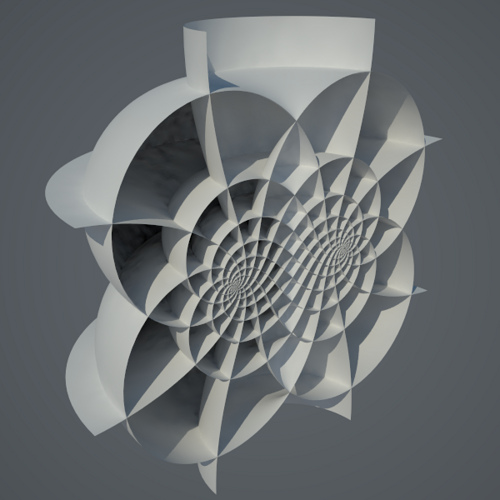
\includegraphics[width=4cm]{triply-orthogonal}
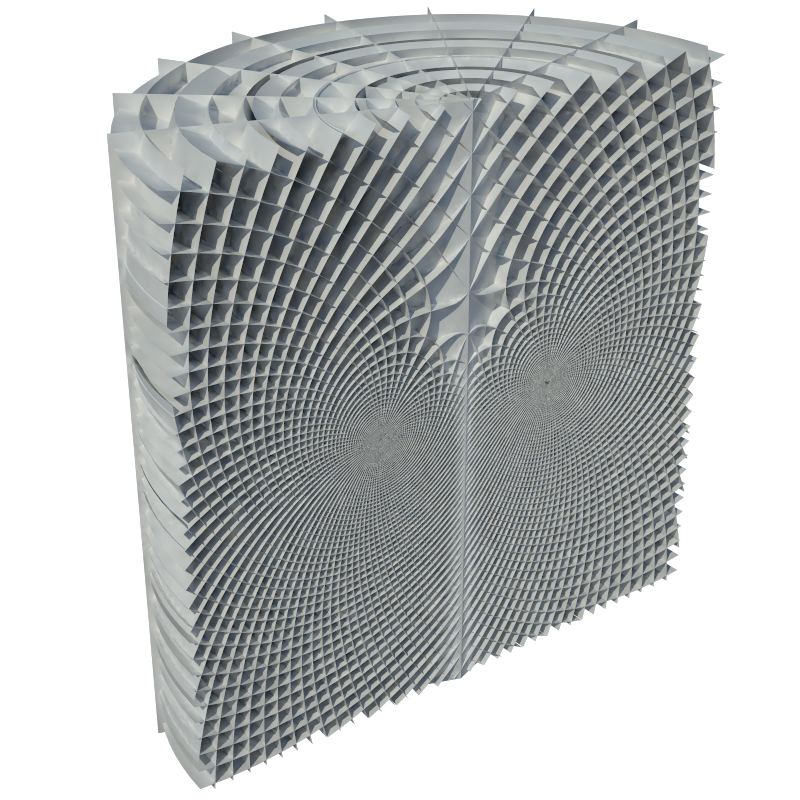
\includegraphics[width=4cm]{triply-orthogonal-web-2b}
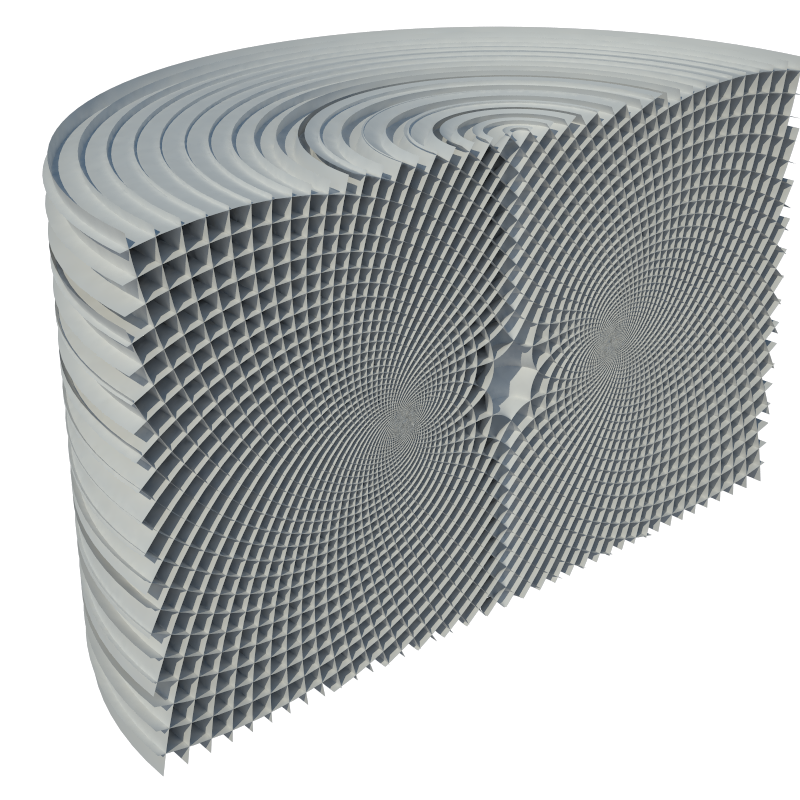
\includegraphics[width=4cm]{triply-orthogonal-web-3}
\par\centering
{\small{Images%(a), (b), (c)
: Daniel Piker, 2015}}\end{list}
\bigskip
\begin{theorem}
There are infinitely many triply orthogonal webs, depending on \(3\) functions of \(2\) variables, defined near any given point of \(3\)-dimensional Euclidean space.
\end{theorem}
\begin{proof}
Picture a triply orthogonal web.
Each leaf is perpendicular to a unique unit length \(1\)-form \(\eta_i\), up to \(\pm\), which satisfies \(0=\eta_i \wedge d \eta_i\), by the Frobenius\SubIndex{Frobenius theorem}\SubIndex{theorem!Frobenius} theorem.
Denote \(3\)-dimensional Euclidean space by \(X\).
Let \(M\) be the set of all orthonormal bases of the tangent spaces of \(X\), with obvious bundle map \(x \colon M \to X\), so that each point of \(M\) has the form \(m=\pr{x,e_1,e_2,e_3}\) for some \(x \in X\) and orthonormal basis \(e_1,e_2,e_3\) of \(T_x X\).
The \emph{soldering \(1\)-forms}\SubIndex{soldering forms} \(\omega_1, \omega_2, \omega_3\) on \(M\) are defined by 
\[
(v \hook \omega_i)e_i = x_* v.
\]
Note: they are \(1\)-forms on \(M\), not on \(X\).
Let 
\[
\omega
\defeq
\begin{pmatrix}
\omega_1 \\
\omega_2 \\
\omega_3
\end{pmatrix}.
\]
As explained in appendix~\ref{chapter:moving.frame}, there is a unique matrix-valued \(1\)-form \(\pi\), valued in antisymmetric \(3 \times 3\) matrices and known as the \emph{Levi-Civita connection},\define{Levi-Civita connection} so that \(d \omega = -\pi \wedge \omega\), i.e.
\[
d
\begin{pmatrix}
\omega_1 \\
\omega_2 \\
\omega_3
\end{pmatrix}
=
-
\begin{pmatrix}
0 & -\pi_3 & \pi_2 \\
\pi_3 & 0 & -\pi_1 \\
-\pi_2 & \pi_1 & 0
\end{pmatrix}
\wedge
\begin{pmatrix}
\omega_1 \\
\omega_2 \\
\omega_3
\end{pmatrix}.
\]
Our triply orthogonal web is precisely a section \(X \to M\) of the bundle map \(M \to X\) on which \(0=\omega_i \wedge d\omega_i\) for all \(i\), hence an integral \(3\)-manifold of the exterior differential system \(\II\) on \(M\) generated by the closed \(3\)-forms
\[
\omega_1 \wedge d \omega_1, \quad
\omega_2 \wedge d \omega_2, \quad
\omega_3 \wedge d \omega_3.
\]
Using the equations above, \(\II\) is also generated by
\[
\pi_3 \wedge \omega_{12}, \quad
\pi_1 \wedge \omega_{23}, \quad
\pi_2 \wedge \omega_{31}.
\]
The integral manifolds coframed by \(\omega_1,\omega_2,\omega_3\) are locally precisely the triply orthogonal webs.
The reader can find the characters: \(s_1,s_2,s_3=0,3,0\), and see that the integral elements coframed by \(\omega_1,\omega_2,\omega_3\) form a manifold of dimension \(12\) (parameterized by choice of a point of \(M\) and \(6\) coefficients to determine values of \(\pi_1,\pi_2,\pi_3\) at each point of \(M\)): involution.
\end{proof}
The reader familiar with Riemannian geometry will note that this proof works just as well for any \(3\)-dimensional Riemannian manifold.
For more on orthogonal webs in Euclidean space, see \cite{Darboux:1993,DeTurck/Yang:1984,Terng/Uhlenbeck:1998,Zakharov:1998}.
\begin{problem*}{eds:Alin}A question of Alin Albu-Sch\"affer: suppose we are given an analytic foliation of an open subset of \(3\)-dimensional Euclidean space by surfaces.
Is there, at least locally, a triply orthogonal web which has this as one of its three foliations?%
\end{problem*}
\begin{answer}{eds:Alin}
Start by looking at the geometry of the given foliation.
Suppose that the foliation is of an open subset \(U\) of \(3\)-dimensional Euclidean space.
Consider the \(4\)-dimensional manifold \(M\) of all orthonormal frames \(e_1,e_2,e_3\) at points \(x\in U\) for which \(e_3\) is perpendicular to the leaf through \(x\) of the given foliation.
By the Frobenius theorem, 
\begin{align*}
0
&=\omega_3\wedge d\omega_3,
\\
&=\omega_3\wedge(\gamma_{13}\wedge\omega_1+\gamma_{23}\wedge\omega_2),
\\
&=
\gamma_{13}\wedge\omega_1\wedge\omega_3+\gamma_{23}\wedge\omega_2\wedge\omega_3.
\end{align*}
So on \(M\),
\[
\begin{pmatrix}
\gamma_{13}\\
\gamma_{23}
\end{pmatrix}
=
\begin{pmatrix}
a_{11}&a_{12}&a_{13}\\
a_{21}&a_{22}&a_{23}
\end{pmatrix}
\begin{pmatrix}
\omega_1\\
\omega_2\\
\omega_3
\end{pmatrix}
\]
for some functions \(a_{ij}\) on \(M\).
Plugging these in above, we find that \(a_{12}=a_{21}\).
Clearly \(a_{11}\omega_1^2+a_{12}\omega_1\omega_2+a_{21}\omega_2\omega_1+a_{22}\omega_2^2\) is the shape operator of each leaf of the foliation.

Now consider the problem of constructing a triply orthogonal web incorporating this foliation as one of its three.
We need to find a choice of \(e_1,e_2\) at each point to construct a frame, so that \(e_1\) will be perpendicular to the leaves of the first foliation, and \(e_2\) perpendicular to the leaves of the second foliation, and the third foliation will be the one we started with, already perpendicular to \(e_3\).
So we will need to solve the exterior differential system
\[
0=\omega_1\wedge d\omega_1=\omega_2\wedge d\omega_2
\]
on \(M\), i.e. with the equations
\[
\begin{pmatrix}
\gamma_{13}\\
\gamma_{23}
\end{pmatrix}
=
\begin{pmatrix}
a_{11}&a_{12}&a_{13}\\
a_{21}&a_{22}&a_{23}
\end{pmatrix}
\begin{pmatrix}
\omega_1\\
\omega_2\\
\omega_3
\end{pmatrix}
\]
already in force.

Note that on \(M\), \(\omega_1,\omega_2,\omega_3,\gamma_{12}\) are linearly independent \(1\)-forms.
We are looking for an integral \(3\)-manifold \(X\) of that exterior differential system, on which we want \(\omega_1,\omega_2,\omega_3\) to be linearly independent, i.e. \(X\) projects by local diffeomorphism to \(3\)-dimensional Euclidean space.

It might be simpler to write our foliation shape operator as
\[
\begin{pmatrix}
\gamma_{13}\\
\gamma_{23}
\end{pmatrix}
=
\begin{pmatrix}
a_{131}&a_{132}&a_{133}\\
a_{231}&a_{232}&a_{233}
\end{pmatrix}
\begin{pmatrix}
\omega_1\\
\omega_2\\
\omega_3
\end{pmatrix}
\]
and then we are imposing only the relations \(a_{132}=a_{231}\), i.e. symmetry in these two outer indices.

Differentiate the equations of our exterior differential system to find that on any integral \(3\)-manifold \(X\):
\begin{align*}
0
&=
\omega_i\wedge d\omega_i,
\\
&=
-\omega_i\wedge\sum_j\gamma_{ij}\wedge\omega_j,
\end{align*}
which forces \(\gamma_{ij}\) to be a linear combination
\[
\gamma_{ij}=\sum_k a_{ijk}\omega_k,
\]
with \(a_{ijk}=-a_{jik}\) since \(\gamma_{ij}=-\gamma_{ji}\).
But plug in to get
\[
0=\omega_i\wedge\sum_{jk}(a_{ijk}-a_{ikj})\omega_k\wedge\omega_j
\]
so that \(a_{ijk}=a_{ikj}\) if \(i,j,k\) are all distinct.
So for distinct indices, \(a_{ijk}\) is symmetric in \(jk\), but antisymmetric in \(ij\).
These two involutions generate the permutation group, and so the sign of \(a_{ijk}\) is a representation of the permutations on \(3\) letters.
But any two involutions are conjugate in the permutation group, so they must force the same sign change.
Hence \(a_{ijk}=0\) for \(i,j,k\) distinct.
This is precisely the demand that the shape operators of the leaves of all three foliations are thus diagonal in the frame \(e_1,e_2,e_3\).
In other words, each leaf of each foliation lies normal to each leaf of each other foliation, and intersects tangent to a principal direction, i.e. along a principal curve.

We can assume that \(U\) is connected.
Either
\begin{enumerate}
\item
the leaves of the given foliation are everywhere umbilic, hence each leaf is an open subset of a sphere or plane, and so \(a_{132}=0\) and \(a_{131}=a_{232}\), or else 
\item
the vectors \(e_1,e_2\) have to be chosen in principal directions and this determines them up to \(4\) choices, at least on a dense open subset of \(U\).
\end{enumerate}

Suppose that the leaves are spheres or planes, so \(a_{132}=0\) and \(a_{131}=a_{232}\), say.
The exterior differential system is generated in dimension \(3\) by \(\gamma_{12}\wedge\omega_1\wedge\omega_2=0\), so every line or plane in any tangent space of \(M\) is an integral element.
Planes, i.e. integral planes, generically have \(\omega_1,\omega_2\) linearly independent on them, so are generically of the form 
\begin{align*}
\gamma_{12}&=p_1\omega_1+p_2\omega_2,\\
\omega_3&=q_1\omega_1+q_2\omega_2,\\
\end{align*}
so lie in a unique \(3\)-dimensional integral element \(\gamma_{12}=p_1\omega_1+p_2\omega_2\).
The polar equations of any integral point or line are trivial, but the generic integral plane has polar equation \(\gamma_{12}-p_1\omega_1-p_2\omega_2\), so \(s_1=0,s_2=1,s_3=0\), solutions depend on \(1\) function of \(2\) variables.

We can explicitly construct the web: take any leaf of our given foliation, the \emph{initial leaf}, and draw on it any foliation by curves.
On that same surface, draw the orthogonal foliation by curves.
Drag each leaf of each of those foliations along the flow of \(e_3\), through space, to trace out a surface.

We want to see that this construction always creates a triply orthogonal web.
Any triply orthogonal web containing the given foliation has to arise from this construction: the leaves of the other two foliations intersect the initial leaf in curves, and the vector field \(e_3\) is tangent to every leaf of the other two foliations.

Conversely, take a foliation of the initial leaf by curves.
Locally pick any orthonormal vector fields \(e_1,e_2\) tangent to that leaf, with \(e_1\) tangent and \(e_2\) perpendicular to that curve foliation.
Drag, as above.
We produce two more foliations of Euclidean space, defined near that leaf.
But it is not clear whether they remain perpendicular.
The leaves of the two new foliations both contain \(e_3\), and they start off perpendicular along the initial leaf.

Compute the change in the Euclidean metric along the flow of \(e_3\):
\[
\LieDer_{e_3} \omega_i\omega_i
=2a_{i3j}\omega_i\omega_j.
\]
So umbilicity of the given leaves is precisely the condition that the Euclidean metric varies only by scaling as we flow along \(e_3\), on the perpendicular vectors to \(e_3\), and so any pair of planes in a tangent space which start perpendicular will remain so.
Hence the construction always succeeds.

Suppose now that the leaves are nowhere umbilic.
We will see that each foliation by nonumbilic surfaces lies in at most one, and typically no, triply orthogonal web.
We need \(e_1,e_2\) to diagonalize the shape operator, i.e. to lie in principal directions.
Imagine drawing the principal curves, i.e. the curves in those directions, on each leaf.
Our given foliation by surfaces has now, on each surface, two foliations by perpendicular curves.
We want to see whether, when we flow along the unit normal vector field \(e_3\) of the foliation, these principal curves flow into one another.
For a generic foliation by surfaces, the flow of \(e_3\) will spin the principal curves of one leaf around into various curves on other leaves, not necessarily principal.

We need \(a_{132}=0\), so the shape operator is diagonalized, i.e. \(e_1,e_2\) point in principal directions, and we suppose the leaves are not umbilic, so \(a_{131}\ne a_{232}\).
Our frames form a \(3\)-manifold \(X\) in the frame bundle.
We have to decide whether \(X\) is an integral manifold.
On \(X\), \(\gamma_{ij}=\sum_k a_{ijk}\omega_k\), for some functions \(a_{ijk}=-a_{jik}\).
To have a triply orthogonal web, we need precisely that \(a_{ijk}=0\) if \(i,j,k\) are distinct, i.e. the shape operators are diagonalized.
This is precisely the condition that the prinicipal curves flow into one another.
\end{answer}


\optionalSection{Generality of integral manifolds}%
If I describe some family of submanifolds as integral manifolds of an exterior differential system, you might find a different description of the same submanifolds as integral manifolds of a different exterior differential system, perhaps on a different manifold, with different characters.
\begin{example} 
A function \(f(x)\) of one variable is equivalent information to having a constant \(f(0)\) and a function \(df/dx\) of one variable.
\end{example}
\begin{example}
We will solve \(\nabla \times u=f-u\) for an unknown vector field \(u\) in \(3\)-dimensional Euclidean space two ways: an elementary approach~\vpageref{page:nabla.u.f.u}, and following Cartan's strategy in problem~\vref{problem:tableaux:nabla}.
The first approach uses \(1\) function of \(1\) variable and \(2\) functions of \(2\) variables.
The second approach uses \(3\) constants, \(3\) functions of \(1\) variable and \(2\) functions of \(2\) variables.
\end{example}
\begin{example}Immersed plane curves are the integral curves of \(\II=0\) on \(M=\R[2]\).
Any integral flag has \(s_0,s_1=0,1\).
Immersed plane curves are also the integral curves of the ideal \(\JJ\) generated by
\[
\vartheta \defeq \sin \phi \, dx - \cos \phi \, dy
\]
on \(M\defeq \R[2]_{x,y} \times S^1_{\phi}\).
Here \(s_0,s_1=1,1\).
\end{example}
\begin{example}
Lagrangian submanifolds of \(\C[n]\) depend on \(1\) function of \(n\) variables: those which are graphs \(y=y(x)\) are of the form
\[
y = \pderiv{S}{x}
\]
for some potential function \(S(x)\), unique up to adding a constant.
On the other hand, the proof of the Cartan--K\"ahler theorem builds up each Lagrangian manifold from a choice of \(1\) function of \(1\) variable, \(1\) function of \(2\) variables, and so on.
\end{example}
We ``trust'' the last nonzero Cartan--K\"ahler \(s_p\) of an involutive exterior differential system to give the generality of integral manifolds: they depend on \(s_p\) functions of \(p\) variables, but we don't ``trust'' \(s_0, s_1, \dots, s_{p-1}\).

\section{What could go wrong?}
\begin{example}
On \(M\defeq\R[3]_{x,y,z}\), take the ideals \(\II\) generated by \(dx\wedge dz, dy\wedge dz\) and \(\JJ\) generated by \(dx\wedge dz, dy\wedge(dz-y \, dx)\).
At the origin, these differential forms are identical, so the integral elements and characters are the same at that point.
But \(\II\) has integral surfaces \(z=\text{constant}\), while \(\JJ\) does not have integral surfaces.
\end{example}
\prob{Wrong}{Compute characters and dimensions of spaces of integral elements for these.
Show that the Cartan--K\"ahler theorem does not apply.
Find their integral surfaces.}

\section{Generalizations}
The Cartan--K\"ahler theorem also holds for holomorphic exterior differential systems on complex manifolds, formal power series exterior differential systems, and Denjoy--Carleman exterior differential systems, with the same proof.
In particular, any involutive smooth exterior differential system is also a formal power series system about each point, so has formal power series solutions,  perhaps divergent.
The theorem also holds for certain smooth systems \cite{Kakie:1989,Kakie:2008,Yang:1987}.